\documentclass[a4paper]{article}
\usepackage[utf8]{inputenc}
\usepackage[czech]{babel}
\usepackage[margin=13mm, tmargin=15mm, bmargin=12mm]{geometry}
\usepackage{multirow}
\usepackage{tikz}
\usetikzlibrary{calc}
\usepackage{chngpage}
\usepackage{tabularx}
\usepackage{fancyhdr}
\usepackage{mathptmx}
\usepackage{lipsum}
\usepackage{float}
\usepackage{longtable}

\renewcommand{\baselinestretch}{1.15}
\pagenumbering{gobble}
\pagestyle{fancy}
\renewcommand{\headrulewidth}{0pt}

\newcommand{\jmeno}{David Škrob, Denis Ku\v{c}era}
\newcommand{\trida}{L3A}
\newcommand{\poradovecislo}{}
\newcommand{\nazevulohy}{LC m\v{e}\v{r}en\'{i}}
\newcommand{\cisloulohy}{}
\newcommand{\predmet}{Technické měření}
\newcommand{\skupina}{}
\newcommand{\datummereni}{8.2.2022}
\newcommand{\datumodevzdani}{16.2.2022}
\newcommand{\klasifikace}{}

\begin{document}
\fancyhead{
\begin{tikzpicture} [overlay,remember picture]
       \draw
        ($ (current page.north west) + (1cm, -12mm) $)
        rectangle
        ($ (current page.south east) + (-1cm,12mm) $);
\end{tikzpicture}
}

\renewcommand{\arraystretch}{2}
\shorthandoff{-}

{
\begin{adjustwidth}[]{-3mm}{-3mm}
\centering
\vspace*{-7mm}
\begin{tabularx}{\linewidth}{l|X|p{3cm}}
\multirow{2}{25mm}{\centering SPŠ a VOŠ technická Brno, Sokolská 1} &
\textbf{LABORATORNÍ CVIČENÍ Z ELEKTROTECHNIKY} & Třída: \trida \\
\cline{2-3}
 & Jméno a příjmení: \jmeno & Poř. Číslo: \poradovecislo \\
\hline
\end{tabularx}

\begin{tabularx}{\linewidth}{X|p{3cm}}
Název úlohy: \nazevulohy & Číslo úlohy: \cisloulohy \\
\hline
Zkoušený předmět: \predmet & Skupina: \skupina \\
\hline
\end{tabularx}

\begin{tabularx}{\linewidth}{X|X|X}
Datum měření: \datummereni &  Datum odevzdání: \datumodevzdani &  Klasifikace: \klasifikace \\
\hline
\end{tabularx}

\end{adjustwidth}
}

\shorthandon{-}

\section*{Zadání}
Změřte kapacitu kondenzátorů podle schémat zapojení v obvodu střídavého sinového napětí o kmitočtu 50 Hz nepřímou metodou.
Výsledky měření zapište do tabulky a zpracujte je matematicky i graficky (do grafu vyneste závislost I = f(U) pro všechny měřené kapacity).
\section*{Vypracování}
\begin{longtable}{c|c|c|c|c|c|c|c}
   	& U [V] & I [mA] & C [uF] & C vypočítané [uF]        & $\Delta$ C [uF]        & $\delta$ C&$\delta$ C [\%]          \\ \endhead
    \hline
	C1 = 0.5 uF & 4 & 0.67  & 0.5 & 0.5331690594 & 0.03316905936 & 0.06221114818&6.22111481\%   \\
	& 8    & 1.34  & 0.5                 & 0.5331690594 & 0.03316905936  & 0.06221114818&6.2211148\%   \\
	& 12   & 2.015 & 0.5                 & 0.5344953506 & 0.03449535055  & 0.06453816767&6.453816767\%   \\
	& 16   & 2.67  & 0.5                 & 0.5311796226 & 0.03117962257  & 0.05869883039&5.86988303\%   \\
	& 20   & 3.18  & 0.5                 & 0.506112719  & 0.006112719032 & 0.01207778189&1.207778189\%   \\
	\hline
	C2 = 2 uF   & 4    & 2.55  & 2                   & 2.029225524  & 0.02922552442  & 0.01440230476&1.440230476\%   \\
	& 8    & 5.11  & 2                   & 2.033204398  & 0.033204398    & 0.01633106737&1.633106737\%   \\
	& 12   & 7.66  & 2                   & 2.031878107  & 0.03187810681  & 0.01568898582&1.568898582\%   \\
	& 16   & 10.21 & 2                   & 2.031214961  & 0.03121496121  & 0.01536763061&1.536763061\%   \\
	& 20   & 12.15 & 2                   & 1.933732559  & 0.06626744143  & 0.03426918637&3.426918637\%   \\
	\hline 
	Cs = 0.4 uF & 4    & 0.53  & 0.4                 & 0.4217605992 & 0.02176059919  & 0.05159467061&5.159467061\%   \\
	& 8    & 1.06  & 0.4                 & 0.4217605992 & 0.02176059919  & 0.05159467061&5.159467061\%   \\
	& 12   & 1.59  & 0.4                 & 0.4217605992 & 0.02176059919  & 0.05159467061&5.159467061\%   \\
	& 16   & 2.12  & 0.4                 & 0.4217605992 & 0.02176059919  & 0.05159467061&5.159467061\%   \\
	& 20   & 2.52  & 0.4                 & 0.4010704566 & 0.001070456592 & 0.00266899886&0.266899886\%   \\
	\newpage \hline
	Cp = 2.5 uF & 4    & 3.22  & 2.5                 & 2.562394584  & 0.06239458378  & 0.02435010758&2.435010758\%   \\
	& 8    & 6.44  & 2.5                 & 2.562394584  & 0.06239458378  & 0.02435010758&2.435010758\%   \\
	& 12   & 9.69  & 2.5                 & 2.570352331  & 0.07035233093  & 0.02737069548&2.737069548\%   \\
	& 16   & 12.89 & 2.5                 & 2.564384021  & 0.06438402057  & 0.02510701207&2.510701207\%   \\
	& 20   & 15.3  & 2.5                 & 2.435070629  & 0.06492937069  & 0.02666426588&2.666426588\%   \\
\end{longtable}

\begin{figure}[H]
	\centering
	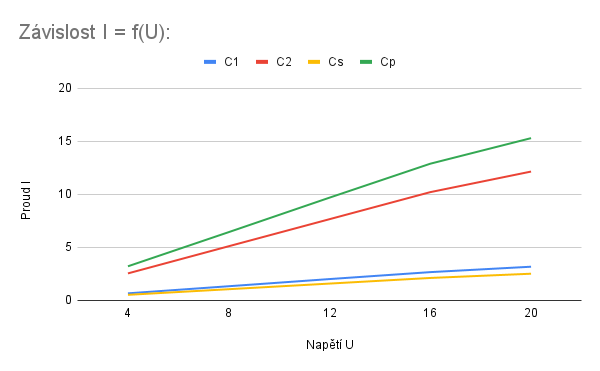
\includegraphics[width=0.75\textwidth]{I_U.png}
	\caption{Graf zavislosti $I$ na $U$}
	\label{fig:mesh1}
\end{figure}

\section*{Zadání}
Změřte nepřímou metodou vlastní indukčnost L cívek L1 a L2.
\section*{Vypracování}
\begin{tabular}{c|c|c|c||c|c|c|c}
	Stejnosměrný & U[V] & I[A] & R[ohm]&& U[V] & I[A] & R[ohm] \\
	\hline
	L1 & 0.71 & 1 & 0.71 & L2 & 3.11 & 1 & 3.11 \\
	& 1.41 & 2 & 0.705 & & 6.12 & 2 & 3.06 \\
	& 2.14 & 3 & 0.71$\overline{3}$ & & 9.15 & 3 & 3.05 \\
	& 2.83 & 4 & 0.7075 & & 12.31 & 4 & 3.0775 \\
	& 3.55 & 5 & 0.71 & & 15.43 & 5 & 3.086 \\
\end{tabular}
\newpage
\begin{tabular}{c|c|c|c|c|c|c}
	Střídavý & R[ohm] & U[V] & I[A] & Z[ohm] & XL[ohm] & L [H] \\ \hline
	L1 & 0.71 & 1.16 & 1 & 1.16 & 1.360036764 & 0.004329131476 \\
	& 0.705 & 2.29 & 2 & 1.145 & 1.344637498 & 0.004280114088 \\
	& 0.7133333333 & 3.42 & 3 & 1.14 & 1.344784163 & 0.004280580938 \\
	& 0.7075 & 4.55 & 4 & 1.1375 & 1.339575492 & 0.004264001225 \\
	& 0.71 & 5.69 & 5 & 1.138 & 1.341321736 & 0.004269559692 \\ \hline
	L2 & 3.11 & 5.1 & 1 & 5.1 & 5.97344959 & 0.01901408059 \\
	& 3.06 & 10.1 & 2 & 5.05 & 5.904752323 & 0.0187954104 \\
	& 3.05 & 15.33 & 3 & 5.11 & 5.95101672 & 0.01894267455 \\
	& 3.0775 & 20.3 & 4 & 5.075 & 5.935202713 & 0.018892337 \\
	& 3.086 & 25.5 & 5 & 5.1 & 5.960989515 & 0.01897441894 \\
\end{tabular}

\section*{Závěr}
Jak mužeme vidět na obrázku \ref{fig:mesh1}, tak když kondenzátory zapojimé seriově, tak se jejich kapacita klesne, což odpovídá námi naměřenými hodnotami proudu a napětí. Dále z obrázku můžeme všimnot, že pokud kondenzátory zapojime paraleně, tak jejich kapacita vzroste, což poznáme na zvýšeném proudu při stejném napětí.\\
\begin{figure}[H]
	\centering
	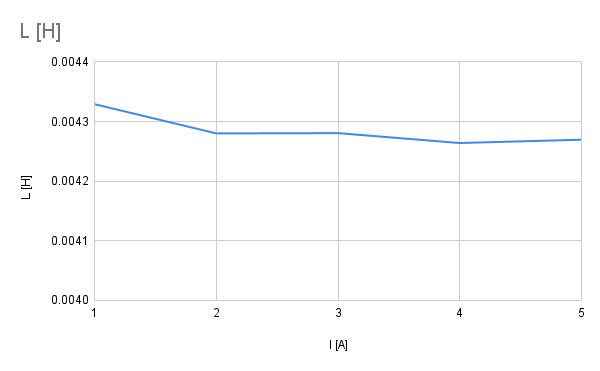
\includegraphics[width=0.75\textwidth]{Lmereni.png}
	\caption{Graf zavislosti $L$ na $I$}
	\label{fig:mesh2}
\end{figure}
Dle obrázku \ref{fig:mesh2} vidíme tendenci kapacitance při vyšším proudu klesat, mohlo by to být způsobené tím, že se cívka při vyšším proudu zahříva, což by mohlo způsobyt tento jev, nebo by za tento jev mohlo snížení přesnosti měření proudu při vyšších proudech. Nebo by za tento jev mohlo moct to, že jsme použili pro výpočet indukce odpor, který jsme změřili při stejném proudu stejnosměrného napětí. Popřípadě by tento jev mohl být pouze statistická odchylka.


\section*{Použité pomucky:}
\begin{tabularx}{\linewidth}{c|c|c|c}
	Přístroj – pomůcka & Typ & Rozsah (pouze analogové)
	& Poznámka \\
	\hline
	Multimetr & Digit\'{a}ln\'{i} &	& \\
	Zdroj st\v{r}\'{i}dav\'{e}ho a stejnosm\v{e}rn\'{e}ho proudu & Zdroj & & \\
	\LaTeX & & & \\
\end{tabularx}
\end{document}